% Copyright (C) 2011 Thomas L. Kula
% All Rights Reserved
%
% See the file LICENSE for license terms.
\documentclass[12pt]{article}
\usepackage{graphicx}
\usepackage{rotating}
\usepackage{fix-cm}
\usepackage{multirow}
\setlength{\paperwidth}{5.5in}
\setlength{\paperheight}{8.5in}
\setlength{\textheight}{7.45in}
\setlength{\topmargin}{-1.0in}
\setlength{\oddsidemargin}{-0.5in}
\setlength{\evensidemargin}{-0.5in}
\setlength{\textwidth}{4.0in}
\setlength{\parindent}{0in}
\setlength{\parskip}{3mm}
\usepackage[print]{booklet} \nofiles
\source{\magstep0}{5.5in}{8.5in}
\target{\magstep0}{11in}{8.5in}
\setpdftargetpages
\pagestyle{empty}
\begin{document}


\begin{center}
{\fontsize{36}{48}\selectfont \textsc{Haiku a Day }}
\end{center}

\vspace*{3.5cm}

{\fontsize{20}{40}\selectfont 


Start placing your bets

For how long it takes me to

Unpack everything

}

\vspace*{5.0cm}
\begin{center}
{\large{Issue 76: October 2011}} \\[5mm]
{\fontsize{8}{8}\selectfont  \textsc{ St. Joshua Norton Press }} \\[1mm]
{\fontsize{6}{6}\selectfont Mathom House by the Cloisters \textbar The People's Republic of Ames }
\end{center}


\newpage

Well folks, here I am, living in New York City. Be sure to check out the new
address on the back cover here. Hopefully next month I'll have all my moving
pictures posted and can provide a link to them.


--- Thomas

http://kula.tproa.net/had/ \\
kula@tproa.net

Download this and previous HADs at the website, so you can
print out your own (DIY, yeah!) or if you want me to send
you one, send me your address, and maybe a stamp if you
are feeling nice. Or send me something you've made ---
trades always appreciated, postcards are nice too.

\vfill

1 October 2011

At Fort Tryon Park \\
Overlooking the Hudson \\
The air flows cooly

2 October 2011

Paint of the ages \\
Softens a bolt's hard edges \\
Layers make hard soft

3 October 2011

A plan is thwarted \\
By a card found expired \\
Columbus later

\newpage

4 October 2011

Brain dump commencing \\
Can I write down all I know? \\
It's time to find out

5 October 2011

Seek apple cider \\
I have too little of it \\
And I must fix that

6 October 2011

Intense sleepyness \\
Too much food and a good beer \\
Bring the land of nod

7 October 2011

A quiet night in \\
Plan on getting up early \\
Muting the night time

8 October 2011

From shelves to boxes \\
A truck driven far away \\
My books will come back

9 October 2011

Interrogation \\
But at least a friendly one \\
Because there was beer

10 October 2011

Such a tiny box \\
In it hours of music \\
I love the future

\newpage

11 October 2011

I need some more tape \\
Yet another thing to go \\
On my to do list

12 October 2011

Ohio Time Warp \\
Three hours to Columbus \\
But five hours back

13 October 2011

How did you get here \\
Wee bug crawling on my desk? \\
Time for you to go.

14 October 2011

Bye computer junk \\
You've filled this garage for years \\
Now you're recycled

15 October 2011

An uneasy dread: \\
Did you forget something, or \\
Forget you forgot?

16 October 2011

Eat way too much food \\
Canadian Thanksgiving \\
Held a week later

17 October 2011

Last minute papers \\
I think I have them all done \\
Better double-check

\newpage

18 October 2011

Boxes consume me \\
Stacks of them, piled on high \\
Taunting, mocking me

19 October 2011

Not much to do here \\
My office packed and empty \\
The last day of work

20 October 2011

No work today, but \\
Still have to get up early \\
Come soon, November

21 October 2011

I am out of room \\
Packing will have to resume \\
When more stuff is gone

22 October 2011

Giant and yellow \\
Lumbering beast growls and starts \\
A vast moving truck

23 October 2011

Now is not the time \\
Sleeping in can come next week \\
For now, we must work

24 October 2011

The list is shrinking \\
I'm sure it will grow again \\
But for now, smaller

\newpage

25 October 2011

Last minutes consume \\
A clock, winding down faster \\
As time passes by

26 October 2011

The big yellow truck \\
Rolling down the road; New York --- \\
What I'm aiming for

27 October 2011

This journey ending \\
Sooner than I expected. \\
Sleep in my new home

28 October 2011

License, PO Box \\
Running all over the place \\
Then I take a nap

29 October 2011

Sorting the boxes \\
Into the rooms they'll go in \\
Enough for today

30 October 2011

Eating out too much \\
I unpack the kitchen and \\
Find a grocery store

31 October 2011

No one at my door \\
Means the candy is all mine. \\
Muahahahaha

\newpage

\begin{center}
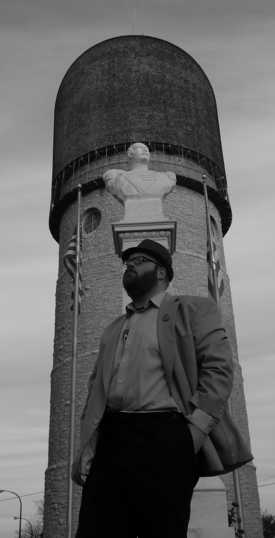
\includegraphics[height=500pt]{thank-you-ypsilant-small.png}

Ypsilanti, Michigan --- 27 October 2011
\end{center}


\newpage

\thispagestyle{empty}
\vspace*{12cm}
\begin{sideways}
\Large{St. Joshua Norton Press}
\end{sideways}
\begin{sideways}
\Large{PO Box 250138}
\end{sideways}
\begin{sideways}
\Large{New York NY 10025}
\end{sideways}


\end{document}


